\chapter{生物体的化学组成}\label{ch:g10:chemistry-of-life}

把一片面包在烤架上烤得太久，它就会变黑：
剩下的主要是碳。称取一片新鲜苹果片的质量，
将其在温暖的烤箱中烘干一天，再次称量：其质量的六分之五以水蒸气形式散失。
面包、苹果、橡树、水母，还有你——每一种生物，
归根结底都由同一小组化学原料构成，
而这份清单不同于构成岩石的清单。本章着手
将生物物质一种成分一种成分地拆开，
探究其独特之处。

\section{元素：与岩石相同的原子，比例却不同}

\begin{definition}[生物物质的化学组成]\label{def:g10:chemistry-of-life:composition}
一份生物物质样本的\emph{化学组成}\index{化学组成}，
是指其中所含化学元素的清单，
以及样本质量中各元素所占的比例。
测定时须对样本进行化学分解——
将其燃烧、称量蒸发掉的部分与残留部分、
分析所释放的气体——而非仅凭观察。
\end{definition}

\begin{proposition}[四种元素占生物体的96\%]\label{prop:g10:chemistry-of-life:four}
按质量计，生物物质几乎完全由四种元素组成：
即氧（O）、碳（C）、氢（H）和氮（N）。在人体中，
它们分别约占质量的 65\%、18.5\%、9.5\% 和 3.2\%，
合计 96\%。钙、磷、钾、硫、钠、
氯和镁占其余 4\% 中的大部分，另有十二种
\emph{微量元素}（铁、锌、碘、铜\dots）
含量远低于 0.1\%，却不可或缺。相同的四种元素
在细菌、小麦植株或鲸鱼体内同样占主导，比例也相近。
\end{proposition}
\admitted

\begin{omfigure}
\begin{tikzpicture}
\begin{axis}[
  ybar, bar width=6pt,
  width=0.92\linewidth, height=6.2cm,
  axis x line=bottom, axis y line=left,
  ymin=0, ymax=75,
  ylabel={质量分数（\%）}, ylabel style={font=\small},
  symbolic x coords={O,C,H,N,Ca,P,Si,Al,Fe},
  xtick=data, tick label style={font=\small},
  enlarge x limits=0.08,
  legend style={at={(0.5,-0.22)}, anchor=north, legend columns=2,
                font=\small, draw=none},
  nodes near coords, nodes near coords style={font=\scriptsize},
  point meta=explicit symbolic,
]
\addplot[fill=omDef!70, draw=omDef] coordinates
  {(O,65) [65] (C,18.5) [18.5] (H,9.5) [9.5] (N,3.2) [3.2] (Ca,1.5) []
   (P,1.0) [1.0] (Si,0.01) [] (Al,0.01) [] (Fe,0.01) []};
\addplot[fill=omProp!70, draw=omProp] coordinates
  {(O,46) [46] (C,0.02) [] (H,0.14) [] (N,0.002) [] (Ca,3.6) [3.6]
   (P,0.1) [] (Si,28) [28] (Al,8.2) [8.2] (Fe,5.6) [5.6]};
\legend{人体, 地壳}
\end{axis}
\end{tikzpicture}

{\small 同样的元素，两种截然不同的“配方”：
人体与地壳岩石中主要元素的质量分数。
（小柱不标数值：钙占人体的 1.5\%；碳占地壳的
0.02\%，氢占 0.14\%，氮占 0.002\%；硅、
铝和铁在人体中仅为痕量）。碳、氢和氮在生物物质中丰富，
在岩石中稀少；硅、铝和铁恰好相反。}
\end{omfigure}

\begin{example}[生物物质与岩石的比较]\label{ex:g10:chemistry-of-life:crust}
地壳中氧也占 46\%，但其余主要元素依次为硅
（28\%）、铝（8\%）和铁（5.6\%）。碳占地壳的 0.02\%，
氮占 0.002\%，而人体中碳和氮分别占 18.5\% 和 3.2\%。生物
因此并非其周围环境的样本：它
\emph{富集}若干元素，倍数达千倍或更多。
这种选择性正是生命的第一个化学特征。
\end{example}

\begin{remark}[原子的来源]\label{rem:g10:chemistry-of-life:origin}
这些原子都很寻常：你肌肉中的碳，
在被植物固定之前是空气中的二氧化碳；你\omterm{def:g10:chemistry-of-life:families}{蛋白质}中的氮，
在被土壤细菌捕获前是空气中的氮。生命的
特殊之处不在原子本身，而在于它们被组装的方式
以及聚集时的比例。
\end{remark}

\section{水与无机盐}

\begin{definition}[无机物与有机物]\label{def:g10:chemistry-of-life:mineral-organic}
生物体内的分子可分为两类。
\emph{无机物}\index{无机物}由一些在生物体外也存在的分子构成，
即水和溶解的
\emph{无机盐}\index{无机盐}（离子，如
$\mathrm{Na^+}$、$\mathrm{K^+}$、$\mathrm{Ca^{2+}}$、$\mathrm{Cl^-}$、
磷酸根和碳酸氢根）。\emph{有机物}\index{有机物}
由以碳原子为骨架、与氢相结合的分子构成，
通常还与氧和氮相结合——这类分子在地球上
只能由生物体或其遗体形成。
\end{definition}

\begin{proposition}[水是主要成分]\label{prop:g10:chemistry-of-life:water}
水是每种生物中含量最多的分子：成年人质量的约 60\%
至 65\%，新生儿为 75\%，苹果为 85\%，
水母为 95\%，而休眠小麦籽粒仅为 13\%。
测定样本含水量的方法是：先称量，
在约 \qty{105}{\celsius} 下烘干至质量不再减少，再次称量：
失去的质量即为水分。
\end{proposition}
\admitted

\begin{example}[烘干苹果片]\label{ex:g10:chemistry-of-life:apple}
一片质量为 \qty{24.0}{g} 的新鲜苹果片，烘干后
质量稳定在 \qty{3.6}{g}。失去的水分：$24.0 - 3.6 = \qty{20.4}{g}$，即
$20.4/24.0 = 0.85$，也就是鲜重的 85\%。剩下的 \qty{3.6}{g}
即\emph{干物质}，包括有机分子和\omterm{def:g10:chemistry-of-life:mineral-organic}{无机盐}。
将干物质燃烧后，剩下约 \qty{0.1}{g} 的浅色灰分——即\omterm{def:g10:chemistry-of-life:mineral-organic}{无机盐}——
得以保留；其余的有机部分，
则以二氧化碳和水蒸气的形式散失。
\end{example}

\begin{omfigure}
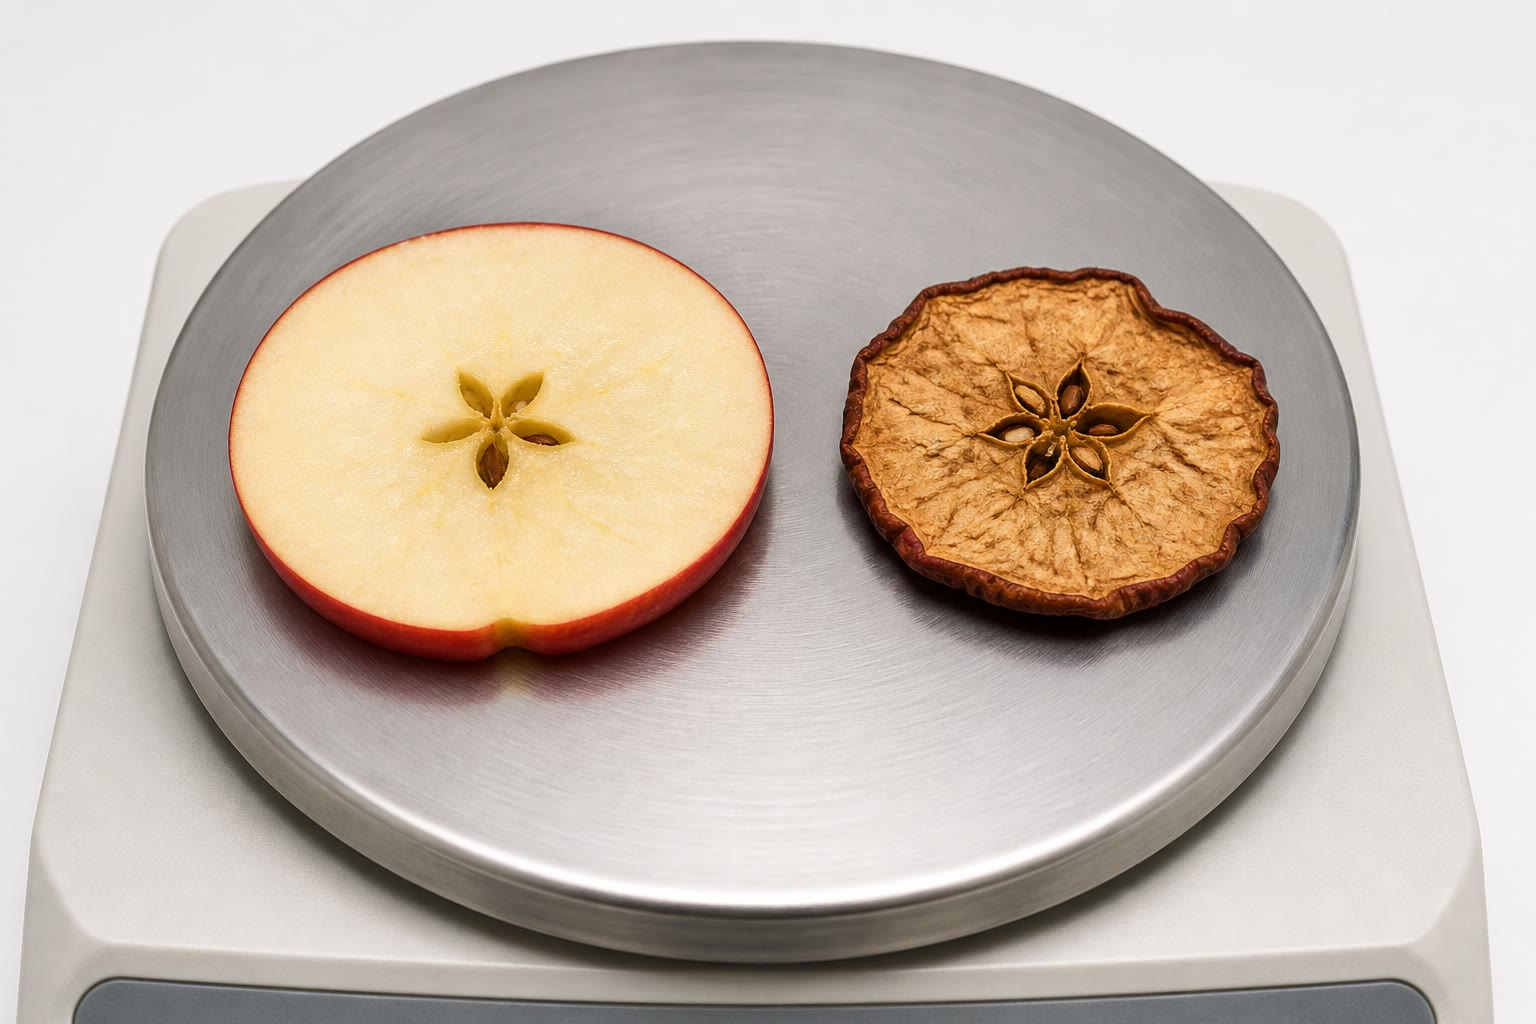
\includegraphics[width=0.56\linewidth]{images/book2/ai/g10-chem-dried-apple.jpg}

{\small 一片新鲜苹果，及其烘干后的样子：
留下的是干物质，约为原质量的六分之一，其余
全是水分。}
\end{omfigure}

\begin{proposition}[水的作用]\label{prop:g10:chemistry-of-life:water-roles}
水是细胞内发生化学反应的场所：它能溶解盐类、
\omterm{def:g10:chemistry-of-life:families}{糖类}以及大多数小分子\omterm{def:g10:chemistry-of-life:mineral-organic}{有机物}，使它们得以相遇并
发生反应；它还能将这些物质从一处运往另一处（血浆中 90\%
是水，汁液中的水分更多）；由于升温需要大量能量，
它能缓冲生物体的温度，使其免受突变的冲击。
体内水分流失 10\%，属于医疗急症；休眠
的种子含水量仅为 13\%，其化学活动只是暂停，
待水分重新回来后才恢复。
\end{proposition}
\admitted

\begin{example}[常见的无机盐]\label{ex:g10:chemistry-of-life:salts}
磷酸钙使骨骼和牙齿变硬（钙约占体重的 1.5\%，
其中几乎全部在骨骼中）。钠离子和氯离子决定了血液的盐度，
接近 \qty{9}{g/L}；钾离子主要
集中在细胞内；铁是血红蛋白的核心成分；
碘是合成甲状腺激素所必需的。\omterm{def:g10:chemistry-of-life:mineral-organic}{无机盐}
本身从不提供能量，但体内一旦缺少其中任何一种，
便会在某项特定任务上出现故障。
\end{example}

\section{有机分子：四大类}

\begin{definition}[糖类、脂质、蛋白质、核酸]\label{def:g10:chemistry-of-life:families}
有机分子分为四大类：
\begin{itemize}
  \item \emph{糖类}\index{糖类}（即糖）只含
        碳、氢和氧三种元素。单糖为单个
        单体，如葡萄糖 $\mathrm{C_6H_{12}O_6}$；复杂的
        糖类是由数百或数千个葡萄糖
        单体连成的长链——植物中为淀粉和纤维素，动物中为糖原。
  \item \emph{脂质}\index{脂质}（如脂肪和油）同样只含
        C、H 和 O，但氧的含量少得多，且不溶
        于水。常见的是甘油三酯，每个甘油三酯由一分子甘油
        与三条长的脂肪酸链相连而成。
  \item \emph{蛋白质}\index{蛋白质}是由
        \emph{氨基酸}\index{氨基酸}组成的链：共二十种氨基酸，均含氮，
        按照精确的顺序连接成
        由五十至数千个单元构成的长链，折叠成
        确定的空间结构。
  \item \emph{核酸}\index{核酸}（DNA 和 RNA）是由
        核苷酸组成的链，除 C、H、
        O 和 N 外还含有磷；它们储存和传递遗传信息，
        并在\cref{ch:g10:universal-dna}中讨论。
\end{itemize}
\end{definition}

\begin{omfigure}
\begin{tikzpicture}[
  box/.style={draw, rounded corners, minimum height=0.9cm, text width=2.6cm,
              align=center, font=\small},
  fam/.style={draw, fill=#1!12, rounded corners, text width=2.6cm, align=center,
              font=\small\bfseries, minimum height=0.8cm,
              text height=1.6ex, text depth=0.4ex},
  >=Stealth]
  \node[fam=omDef] (c) at (0,0) {糖类};
  \node[fam=omProp] (l) at (3.2,0) {脂质};
  \node[fam=omThm] (p) at (6.4,0) {蛋白质};
  \node[fam=omMeth] (n) at (9.6,0) {核酸};
  \node[box] (cu) at (0,-1.7) {单体：葡萄糖 \\ $\mathrm{C_6H_{12}O_6}$};
  \node[box] (lu) at (3.2,-1.7) {单体：甘油 \\ + 脂肪酸};
  \node[box] (pu) at (6.4,-1.7) {单体：20 种 \\ 氨基酸};
  \node[box] (nu) at (9.6,-1.7) {单体：4 种 \\ 核苷酸};
  \node[box] (cp) at (0,-3.6) {淀粉、糖原、\\ 纤维素};
  \node[box] (lp) at (3.2,-3.6) {甘油三酯、\\ 膜脂质};
  \node[box] (pp) at (6.4,-3.6) {酶、纤维、\\ 抗体};
  \node[box] (np) at (9.6,-3.6) {DNA, RNA};
  \foreach \a/\b in {c/cu, l/lu, p/pu, n/nu} \draw (\a) -- (\b);
  \foreach \a/\b in {cu/cp, lu/lp, pu/pp, nu/np}
    \draw[->] (\a) -- node[right, font=\scriptsize] {链} (\b);
  \node[font=\small, anchor=east] at (-1.6,-1.7) {单体};
  \node[font=\small, anchor=east] at (-1.6,-3.6) {大分子};
\end{tikzpicture}

{\small 有机分子的四大类。每个大分子都是
由小单体连接而成的链；单体的种类，以及
链的排列方式，决定了分子的作用。}
\end{omfigure}

\begin{example}[读懂食品标签]\label{ex:g10:chemistry-of-life:label}
全麦面包的标签上标明，每 \qty{100}{g}：\omterm{def:g10:chemistry-of-life:families}{糖类}
\qty{41}{g}（其中糖 \qty{3}{g}）、脂肪 \qty{3}{g}、\omterm{def:g10:chemistry-of-life:families}{蛋白质}
\qty{9}{g}、纤维 \qty{7}{g}、盐 \qty{1.1}{g}。其余部分——约
\qty{39}{g}——是水。标签上的“\omterm{def:g10:chemistry-of-life:families}{糖类}”主要是淀粉，“糖”
指的是单糖，“纤维”是纤维素（一种我们无法消化的\omterm{def:g10:chemistry-of-life:families}{糖类}）
，“脂肪”指\omterm{def:g10:chemistry-of-life:families}{脂质}，“盐”指\omterm{def:g10:chemistry-of-life:mineral-organic}{无机盐}。标签是
经过取整的化学分析。
\end{example}

\begin{proposition}[各类分子的作用]\label{prop:g10:chemistry-of-life:roles}
四大类分子分担细胞的工作，且功能有交叉：
\begin{itemize}
  \item \omterm{def:g10:chemistry-of-life:families}{糖类}是日常的燃料（葡萄糖），其短期储备为
        淀粉和糖原，纤维素则是
        植物细胞壁的构件；
  \item \omterm{def:g10:chemistry-of-life:families}{脂质}是紧凑的长期能量储存（每克 \qty{38}{kJ}，
        \omterm{def:g10:chemistry-of-life:families}{糖类}和\omterm{def:g10:chemistry-of-life:families}{蛋白质}则为每克 \qty{17}{kJ}），
        膜\omterm{def:g10:chemistry-of-life:families}{脂质}构成每个细胞的包膜；
  \item \omterm{def:g10:chemistry-of-life:families}{蛋白质}是细胞的“机器”：催化每一步反应的酶、
        使肌肉收缩的纤维、载体、抗体、
        受体；
  \item \omterm{def:g10:chemistry-of-life:families}{核酸}保存着构建\omterm{def:g10:chemistry-of-life:families}{蛋白质}的指令。
\end{itemize}
\end{proposition}
\admitted

\begin{omfigure}
\begin{tikzpicture}
\begin{axis}[
  xbar stacked, bar width=14pt,
  width=0.9\linewidth, height=3.2cm,
  axis x line=bottom, axis y line=none,
  xmin=0, xmax=100,
  xtick={0,20,40,60,80,100}, tick label style={font=\small},
  ytick=\empty, enlarge y limits=0.6,
  legend style={at={(0.5,-0.45)}, anchor=north, legend columns=5,
                font=\small, draw=none, column sep=4pt},
]
\addplot[fill=omDef!35, draw=omDef] coordinates {(60,0)};
\addplot[fill=omThm!45, draw=omThm] coordinates {(17,0)};
\addplot[fill=omProp!45, draw=omProp] coordinates {(16,0)};
\addplot[fill=gray!35, draw=gray] coordinates {(6,0)};
\addplot[fill=omMeth!55, draw=omMeth] coordinates {(1,0)};
\legend{水 60, 蛋白质 17, 脂质 16, 无机盐 6, 糖类 1}
\end{axis}
\end{tikzpicture}

{\small 成年人体按质量计的组成（百分比）。数值
随年龄与体型而变（瘦削的运动员\omterm{def:g10:chemistry-of-life:families}{脂质}较少，新生儿水分较多），
但水始终占主导，游离\omterm{def:g10:chemistry-of-life:families}{糖类}
从不超过约 1\%。}
\end{omfigure}

\begin{remark}[大分子与生命的形态]\label{rem:g10:chemistry-of-life:macromolecules}
岩石中的分子小而重复（石英晶体为
无尽重复的 $\mathrm{SiO_2}$）。生命特有的分子
极其庞大——单个\omterm{def:g10:chemistry-of-life:families}{蛋白质}可含上万个原子，一个
DNA 分子可含数十亿个原子——而且\emph{携带信息}：其
构件的排列顺序承载着信息。矿物世界中
没有任何东西类似于序列有意义的分子。
\end{remark}

\section{鉴定组成成分}

\begin{method}[各类物质的标准检测方法]\label{met:g10:chemistry-of-life:tests}
每类物质都有一种简单的检验方法，能给出可见的结果。
\begin{enumerate}
  \item \emph{水}：一条蓝色的氯化钴试纸变为粉红色；
        或将样品烘干并测量失去的质量。
  \item \emph{淀粉}：一滴碘液由
        棕黄色变为蓝黑色。
  \item \emph{单糖}（葡萄糖、果糖\dots）：与
        斐林试剂或本尼迪特试剂共热；蓝色溶液
        生成砖红色沉淀。
  \item \emph{\omterm{def:g10:chemistry-of-life:families}{蛋白质}}：双缩脲检验——加入几滴
        碱性硫酸铜溶液，样品变为紫色。
  \item \emph{\omterm{def:g10:chemistry-of-life:families}{脂质}}：样品在纸上留下半透明、不干的斑点；
        红色染料苏丹 III 可使其着色。
  \item \emph{\omterm{def:g10:chemistry-of-life:mineral-organic}{无机盐}}：将干物质充分燃烧，残留的灰分
        即为\omterm{def:g10:chemistry-of-life:mineral-organic}{无机物}。特定离子可通过
        沉淀反应鉴定（例如用硝酸银检测氯离子）。
\end{enumerate}
始终应设置对照：一组使用纯水，
另一组使用已知的阳性样品，以确认试剂有效，
并确保颜色变化确实表示你所判断的结果。
\end{method}

\begin{example}[分析土豆]\label{ex:g10:chemistry-of-life:potato}
生土豆片：氯化钴试纸变为粉红色（水）；碘液
立即变为蓝黑色（淀粉，含量丰富）；斐林试剂仅
产生微弱的橙色（游离糖很少）；双缩脲检验呈淡紫色
（含有一定量\omterm{def:g10:chemistry-of-life:families}{蛋白质}，约占鲜重的 2\%）；无半透明斑点
（几乎不含\omterm{def:g10:chemistry-of-life:families}{脂质}）。烘干后剩余质量的 22\%；燃烧后
残留灰分占 1\%。土豆是包裹在水中的淀粉储备——
正是植物在冬季地下存活所需要的。
\end{example}

\begin{proposition}[组成的统一性]\label{prop:g10:chemistry-of-life:unity}
无论何种生物体——细菌、蘑菇、植物、动物——
同样的检验都会发现相同的四类物质，它们由相同的
构件组成：相同的二十种\omterm{def:g10:chemistry-of-life:families}{氨基酸}、相同的葡萄糖、相同的四种
核苷酸。生物的独特之处并不在于拥有特殊的原子
或特殊的构件，而在于它所维持的比例、它所组装的
超大分子，以及这些分子所携带的
信息。这种化学上的统一性，是支持所有生物
拥有共同起源的最有力论据之一，这一论证将在
\cref{ch:g10:common-ancestry}中展开。
\end{proposition}
\admitted

\begin{omfigure}
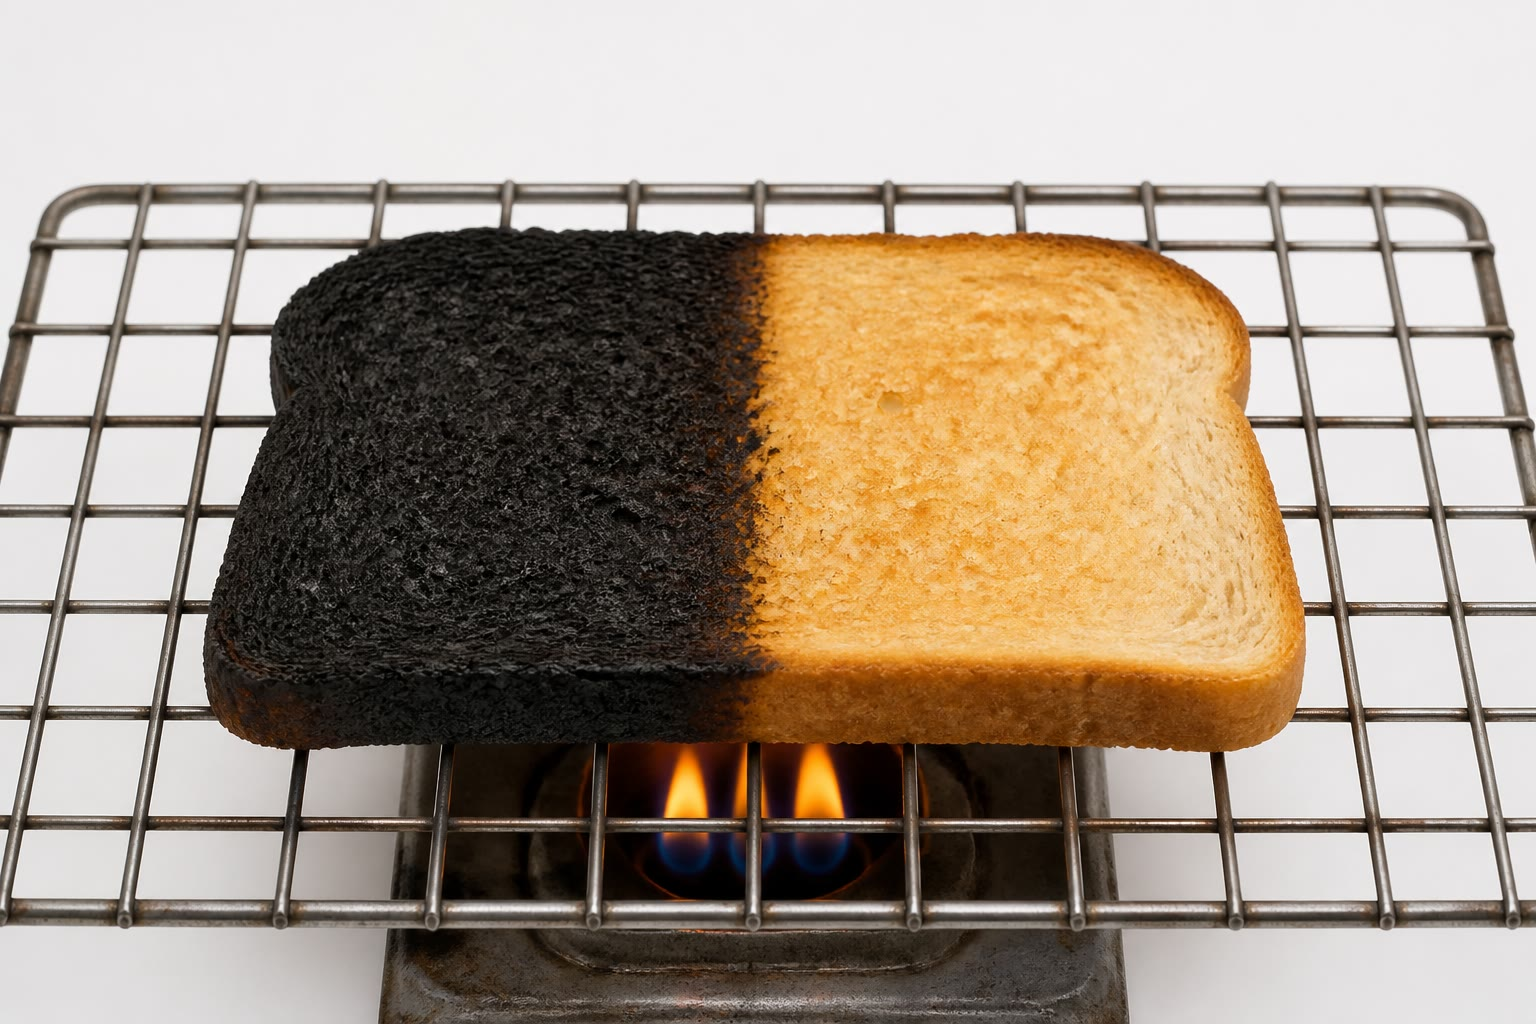
\includegraphics[width=0.6\linewidth]{images/book2/ai/g10-chem-charred-bread.jpg}

{\small 烤架上的面包烤过了头。黑色残留物主要是
碳：面包中的有机分子失去了氢和
氧，以水蒸气和二氧化碳的形式散失，
只留下碳骨架。}
\end{omfigure}

\section{练习}

\begin{exercise}[$\star$]\label{exo:g10:chemistry-of-life:1}
写出构成生物体质量 96\% 的四种元素，
并给出其在人体中的大致百分比。
\end{exercise}

\begin{exercise}[$\star$]\label{exo:g10:chemistry-of-life:2}
将下列物质分为\omterm{def:g10:chemistry-of-life:mineral-organic}{无机物}与\omterm{def:g10:chemistry-of-life:mineral-organic}{有机物}：水、葡萄糖、氯化钠、
甘油三酯、磷酸钙、\omterm{def:g10:chemistry-of-life:families}{氨基酸}、
二氧化碳。
\end{exercise}

\begin{exercise}[$\star$]\label{exo:g10:chemistry-of-life:3}
一片质量为 \qty{12.0}{g} 的新鲜生菜叶被烘干至
恒定质量：\qty{0.6}{g}。求其含水量（以百分数表示）。
\end{exercise}

\begin{exercise}[$\star$]\label{exo:g10:chemistry-of-life:4}
哪种检验可用来证明一粒豆种子含有（a）淀粉、
（b）\omterm{def:g10:chemistry-of-life:families}{蛋白质}、（c）\omterm{def:g10:chemistry-of-life:families}{脂质}？分别给出各情况下的预期结果。
\end{exercise}

\begin{exercise}[$\star$]\label{exo:g10:chemistry-of-life:5}
写出每类物质的基本组成单位：\omterm{def:g10:chemistry-of-life:families}{糖类}、\omterm{def:g10:chemistry-of-life:families}{脂质}、
\omterm{def:g10:chemistry-of-life:families}{蛋白质}、\omterm{def:g10:chemistry-of-life:families}{核酸}。
\end{exercise}

\begin{exercise}[$\star\star$]\label{exo:g10:chemistry-of-life:6}
利用本章第一幅图，碳在人体中的含量是地壳中的多少倍？
氮呢？
请加以说明。
\end{exercise}

\begin{exercise}[$\star\star$]\label{exo:g10:chemistry-of-life:7}
一名质量为 \qty{70}{kg} 的成年人，体内含水 62\%。求其体内水的质量，
再求干物质的质量。若\omterm{def:g10:chemistry-of-life:families}{蛋白质}占体重的 17\%，
则\omterm{def:g10:chemistry-of-life:families}{蛋白质}的质量为多少？
\end{exercise}

\begin{exercise}[$\star\star$]\label{exo:g10:chemistry-of-life:8}
一根谷物棒每 \qty{100}{g} 含\omterm{def:g10:chemistry-of-life:families}{糖类} \qty{60}{g}、
\omterm{def:g10:chemistry-of-life:families}{脂质} \qty{12}{g} 和\omterm{def:g10:chemistry-of-life:families}{蛋白质} \qty{8}{g}。利用
\cref{prop:g10:chemistry-of-life:roles}中的能量值，求
\qty{100}{g} 该谷物棒提供的能量，以及
其中来自\omterm{def:g10:chemistry-of-life:families}{脂质}的比例。
\end{exercise}

\begin{exercise}[$\star\star$]\label{exo:g10:chemistry-of-life:9}
分别向一片面包、一片奶酪和
一块糖中滴加碘液。预测每种情况下的结果并加以解释。
\end{exercise}

\begin{exercise}[$\star\star$]\label{exo:g10:chemistry-of-life:10}
为什么植物干物质能够燃烧，而其留下的灰分
却不能？二者各属于哪一类物质？
\end{exercise}

\begin{exercise}[$\star\star$]\label{exo:g10:chemistry-of-life:11}
已知两种溶液，一种为葡萄糖溶液，一种为淀粉溶液。斐林
试剂检测仅对前者呈阳性，碘液仅对后者呈阳性。然而淀粉
是由葡萄糖构成的。请提出一种解释。
\end{exercise}

\begin{exercise}[$\star\star\star$]\label{exo:g10:chemistry-of-life:12}
一粒小麦籽粒含水 13\%；萌发三天后的幼苗含水
88\%。请解释这一变化，并说明它反映出水在种子
化学过程中的作用。
\end{exercise}

\begin{exercise}[$\star\star\star$]\label{exo:g10:chemistry-of-life:13}
血浆中约含氯化钠 \qty{9}{g/L}，
约含葡萄糖 \qty{1}{g/L}。某患者接受了 \qty{500}{mL}
静脉输注溶液。该溶液中氯化钠与葡萄糖的质量
应为多少，才能与血浆相匹配？为什么纯水会有危险？
\end{exercise}

\begin{exercise}[$\star\star\star$]\label{exo:g10:chemistry-of-life:14}
\omterm{def:g10:chemistry-of-life:families}{脂质}的储能为 \qty{38}{kJ/g}，糖原为 \qty{17}{kJ/g}；此外，
体内每克糖原约与 \qty{3}{g} 水一同储存。
某人体内储有 \qty{0.5}{kg} 糖原和 \qty{10}{kg} \omterm{def:g10:chemistry-of-life:families}{脂质}。
求每种储能物质所含的能量，以及人体若以含水糖原形式
储存与\omterm{def:g10:chemistry-of-life:families}{脂质}等量能量所需携带的质量。并由此推断
动物为何要储存脂肪。
\end{exercise}

\begin{exercise}[$\star\star\star$]\label{exo:g10:chemistry-of-life:15}
“生物与岩石由相同的原子组成，因此
生命在化学上并无任何特殊之处。”请用一个短段落讨论这一论断，
并运用本章中的三条准确论据加以说明。
\end{exercise}

\section{问题：人体中的碳}

\begin{problem}[{周末问题——从麦田到人体：物质的核算，
从一粒籽粒中的水，到一个人所携带的碳的千克数
}]
\label{pb:g10:chemistry-of-life:1}
一个班级追踪物质从麦田转移到其中一名学生身体的全过程。
数据：一粒小麦籽粒含水 13\%，其干物质中
约含淀粉 70\%、\omterm{def:g10:chemistry-of-life:families}{蛋白质} 12\%、\omterm{def:g10:chemistry-of-life:families}{脂质} 2\%、矿物质 2\%，其余为
纤维素。面包用的面粉大致保持籽粒内部的
组成。学生莉亚的质量为 \qty{60}{kg}；使用
第二幅图中成年人的组成（水 60\%、\omterm{def:g10:chemistry-of-life:families}{蛋白质} 17\%、
\omterm{def:g10:chemistry-of-life:families}{脂质} 16\%、矿物质 6\%、\omterm{def:g10:chemistry-of-life:families}{糖类} 1\%）。各类物质中各元素的
质量分数取值：\omterm{def:g10:chemistry-of-life:families}{糖类}含碳 40\%，\omterm{def:g10:chemistry-of-life:families}{脂质}含碳 77\%，
\omterm{def:g10:chemistry-of-life:families}{蛋白质}含碳 53\%、含氮 16\%。

\medskip
\noindent\textbf{第一部分——籽粒。}
\begin{enumerate}
  \item 一粒质量为 \qty{45}{mg} 的籽粒被烘干。
        它失去的水的质量是多少，其干质量为多少？
  \item 计算一粒籽粒干物质中的
        淀粉、\omterm{def:g10:chemistry-of-life:families}{蛋白质}和\omterm{def:g10:chemistry-of-life:families}{脂质}的质量。
  \item \cref{met:g10:chemistry-of-life:tests}中的哪些检验可用于
        验证磨碎的籽粒中这三种成分？
  \item 籽粒播种并浇水；三天后幼苗含水
        88\%。请解释为何在含水 13\% 时萌发不能开始。
  \item 一公顷产量为 \qty{8}{t} 籽粒，随之收获的水的质量是多少，
        干物质的质量又是多少？
\end{enumerate}

\medskip
\noindent\textbf{第二部分——面包。}
\begin{enumerate}[resume]
  \item 一个面包用 \qty{500}{g} 面粉、\qty{320}{g} 水和
        \qty{10}{g} 盐烘焙制成，烘焙中失去 \qty{130}{g} 水。
        烘焙后面包的质量是多少，其
        含水量为百分之几？
  \item 以籽粒的干物质组成代表面粉，估算
        面包中淀粉和\omterm{def:g10:chemistry-of-life:families}{蛋白质}的质量。
  \item \omterm{def:g10:chemistry-of-life:families}{糖类}和\omterm{def:g10:chemistry-of-life:families}{蛋白质}按 \qty{17}{kJ/g}、\omterm{def:g10:chemistry-of-life:families}{脂质}按
        \qty{38}{kJ/g} 计算，估算面包所含的
        能量。
  \item 莉亚食用 \qty{120}{g} 该面包，其提供的能量占每日
        约 \qty{10000}{kJ} 需要量的比例是多少？
  \item 面包中的盐为何不是能量来源，它在
        人体中起什么作用？
\end{enumerate}

\medskip
\noindent\textbf{第三部分——人体：水与三大类分子。}
\begin{enumerate}[resume]
  \item 计算莉亚体内水的质量。
  \item 计算\omterm{def:g10:chemistry-of-life:families}{蛋白质}、\omterm{def:g10:chemistry-of-life:families}{脂质}、矿物质和\omterm{def:g10:chemistry-of-life:families}{糖类}的质量。
  \item 莉亚在一次长跑中出汗失去 \qty{1.2}{kg} 水分。
        这占她体内水分的比例为多少？为何必须
        迅速补充？
  \item 她的血液约 \qty{4.5}{L}，其中血浆占 55\%，
        血浆中 90\% 为水。估算她血液中水的质量（按
        每升 \qty{1}{kg} 计）。这占她体内水分的比例为多少？
        其余的水在哪里？
  \item 新生儿的含水量为 75\%。请用一句话解释，为何婴儿
        比成人更容易脱水。
\end{enumerate}

\medskip
\noindent\textbf{第四部分——人体：元素。}
\begin{enumerate}[resume]
  \item 利用每类分子中的碳含量，计算莉亚体内
        \omterm{def:g10:chemistry-of-life:families}{糖类}、\omterm{def:g10:chemistry-of-life:families}{脂质}和\omterm{def:g10:chemistry-of-life:families}{蛋白质}中碳的质量，再计算
        碳的总质量。
  \item 碳占她体重的比例为多少？请与
        \cref{prop:g10:chemistry-of-life:four}中的 18.5\% 比较，并评论
        两者是否一致。
  \item 计算她\omterm{def:g10:chemistry-of-life:families}{蛋白质}中氮的质量。这些氮最终
        来自何处？
  \item 按质量计，水中 89\% 为氧。计算仅由她体内水所携带的氧
        的质量，并与 65\% 比较，该数值见
        \cref{prop:g10:chemistry-of-life:four}。哪一种分子
        解释了体内大部分的氧？
  \item 用一句话说明结果：一个 \qty{60}{kg} 的人，
        体内携带多少千克碳，并通过哪两个
        生物学过程使这些碳离开空气
        进入人体？
\end{enumerate}
\end{problem}
